\section{Method of Interpolating Differences between Approximate Solutions (MIDAS)} \label{sec:MIDAS}
In this section, we present a method called MIDAS to reduce the overall computational cost when POEM is applied. We first study the distribution of shared grid points in the domain when fractional refinement ratios are used. Then, we address its relation to the computational cost and propose how to increase the number of shared grid points. Lastly, we show that MIDAS does not have a significant effect on the estimated DE.

%------------------------------------------------------------------------------

\subsection{Distribution of Shared Grid Points in Fractional Refinement}
When we try to apply POEM to local system quantities over the entire domain, we need to know the distribution of the \textit{shared grid points}, i.e. the common locations of grid points on different refinement levels. In the case of grid doubling ($r=0.5$), a shared grid point is located at each grid point on the coarser grid and alternately resides on the finer grid. However, in the case of refinement ratios greater than 0.5, this distribution is not obvious.

To simplify the problem, we restricted ourselves to the study of systematic grid refinement for Cartesian grids. This means that the grid spacing is uniform on each refinement level and that the same refinement ratio is applied throughout the domain \citep{Roy2010}. In addition, we introduce the concept of an \textit{irreducible unit} which is defined in Definition \ref{def:IU} and illustrated in Figure \ref{fig:setG}.
\begin{definition} \label{def:IU}
    Let $G$ be a set of systematically-refined grids with uniform grid spacing. An irreducible unit of $G$ is the smallest repeating unit in $G$.
\end{definition}

\begin{figure}[!htb]
\centering
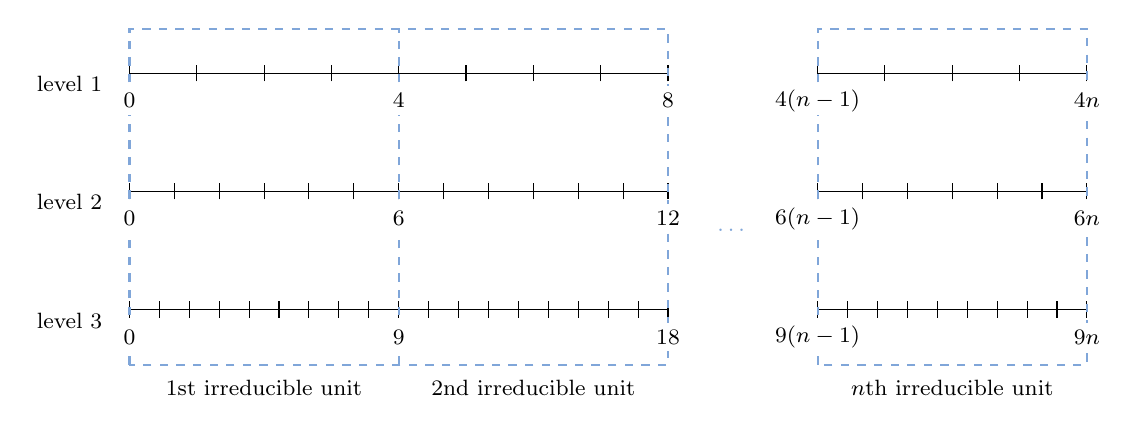
\begin{tikzpicture}[
    xscale=0.38,
    %yscale=1,
    font=\footnotesize,
    bx/.style={color=blue!70!green!50, thick, dashed}
]
    % Loop over start positions
    \foreach \st in {0,9,23}{
        % Draw grids
        \draw (\st, 3.0) -- (\st + 9, 3.0);
        \draw (\st, 1.5) -- (\st + 9,1.5);
        \draw (\st, 0.0) -- (\st + 9,0.0);
    
        \foreach \x in {0,...,4}{
            \draw ({\st + \x*9/4}, 3.0cm - 3pt) -- ({\st + \x*9/4}, 3.0cm + 3pt);
        }
        \foreach \x in {0,...,6}{
            \draw ({\st + \x*9/6}, 1.5cm - 3pt) -- ({\st + \x*9/6}, 1.5cm + 3pt);
        }
        \foreach \x in {0,...,9}{
            \draw ({\st + \x}, -3pt) -- ({\st + \x}, 3pt);
        }
    }
    
    % Draw ellipsis
    \node[bx] at (20cm + 5pt, 1.0) {\ldots};
    
    % Draw boxes (bottom layer)
    \draw[bx] (0, 0cm - 20pt) rectangle (18, 3.0cm + 16pt);
    \draw[bx] (9, 0cm - 20pt) -- (9, 3.0cm + 16pt);
    \draw[bx] (23, 0cm - 20pt) rectangle (23 + 9, 3.0cm + 16pt);
    
    % Draw boxes to cover the lines (middle layer)
    \foreach \st in {0,9,18,23,32}{
        \foreach \y in {3.0,1.5,0.0}{
            \draw[color=white, fill=white] (\st*1cm - 5pt, \y*1cm - 10pt - 5pt) rectangle (\st*1cm + 5pt, \y*1cm - 10pt + 5pt);
        }
    }
    
    % Label indices (top layer)
    \foreach \x in {0,4,8}{
        \node at (\x*9/4, 3.0cm - 10pt) {$\x$};
    }
    \foreach \x in {0,6,12}{
        \node at (\x*9/6, 1.5cm - 10
        pt) {$\x$};
    }
    \foreach \x in {0,9,18}{
        \node at (\x, -10pt) {$\x$};
    }
    \node at (23 + 0, {3.0 cm - 10pt}) {$4(n-1)$};
    \node at (23 + 9, {3.0 cm - 10pt}) {$4n$};
    \node at (23 + 0, {1.5 cm - 10pt}) {$6(n-1)$};
    \node at (23 + 9, {1.5 cm - 10pt}) {$6n$};
    \node at (23 + 0, {0.0 cm - 10pt}) {$9(n-1)$};
    \node at (23 + 9, {0.0 cm - 10pt}) {$9n$};
    
    % Label units
    \node at ({0 + 4.5}, -1) {1st irreducible unit};
    \node at ({9 + 4.5}, -1) {2nd irreducible unit};
    \node at ({23 + 4.5}, -1) {$n$th irreducible unit};
    
    % Label levels
    \node at (-2, 3.0cm - 4pt) {level 1};
    \node at (-2, 1.5cm - 4pt) {level 2};
    \node at (-2, 0.0cm - 4pt) {level 3};
    
\end{tikzpicture}
\caption{Schematic diagram of $G$ consisting of three grid levels characterized by a refinement ratio of $\frac{2}{3}$. The margin of irreducible units are depicted by dashed lines.}
\label{fig:setG}
\end{figure}

Definition \ref{def:IU} is made in such a way that a shared grid point resides only at the margins of an irreducible unit, thus reducing the complexity of the problem. Nevertheless, an irreducible unit is still hypothetical up to this point. We now propose the following.

\begin{proposition} \label{prop:IU_u&e}
    Let $S_l$ be the number of grid segments on the $l$th level of $G$, and let $s_l$ be the number of grid segments on the $l$th level of the irreducible unit. Also, denote $gcd(\cdot)$ the greatest common divisor of a set of integers. Then an irreducible unit of $G$ exists and is unique. Furthermore, the irreducible unit repeats $gcd(\{S_l\})$ times in $G$ and $s_l = S_l/gcd(\{S_l\})$.
\end{proposition}
\begin{proof}
    From the theory of numbers, the greatest common divisor of two integers exists and is unique \citep{Tattersall2005}. This is also true for multiple integers since $gcd(S_1,S_2,S_3) = gcd(gcd(S_1,S_2),S_3)$. So is $gcd(\{S_l\})$. Therefore, $G$ can be divided into at most $gcd(\{S_l\})$ identical units, which are exactly the irreducible units. Furthermore, every unit contains $S_l/gcd(\{S_l\})$ segments at the $l$th level.
\end{proof}

From Definition \ref{def:IU} and Proposition \ref{prop:IU_u&e}, it follows that if two sets of grids contain the same number of refinement levels and are characterized by the same refinement ratio, then they are identified by the same irreducible unit. In addition, the knowledge that the irreducible unit repeats in a simulation domain is useful for programming: operations over the domain can be implemented by applying the operations on an irreducible unit in each iteration and advancing in a step size of the irreducible unit.

With the concept of irreducible units, we can examine what forms of $r$ maximize the proportion of shared grid points in $G$. Consider a set of two-level irreducible units characterized by various $\{s_1,s_2\}$. Since a shared grid point resides only at the margins, these units must contain the same number of shared grid points. What affects the proportion is the number of interior grid points. Since any additional point in the interior grid will lower the proportion, the lowest proportion is attained when the next refinement level contains one more point in the interior grid than the current level, i.e. $s_2 = s_1 + 1$. Therefore, to maximize the proportion of shared grid points, one should choose refinement ratios of the form $r = s_1 / (s_1 + 1)$, which are referred to as \textit{fractional refinement ratios}. We can further deduce that the grid doubling, where $r=0.5$ and $s_1=1$, corresponds to the maximum proportion.

%------------------------------------------------------------------------------

\subsection{Creating Shared Grid Points by Interpolation} \label{subsec:interp}
If fractional refinement is applied, the targets of POEM, $\Tilde{\phi}_{e}$ and $\{C_{p}h^p\}$, will be sparser in the domain compared to grid doubling. Consequently, the estimated DE will contain a larger statistical error due to the smaller sample size, i.e. $N$ in Equation \ref{eq:L1_norm} -- \ref{eq:L8_norm}. While it seems to be a trade-off between the computational cost and the confidence of the results, MIDAS can be used to compensate the increased uncertainty by adding shared grid points to the domain.

According to Proposition \ref{prop:IU_u&e}, the boundaries of an irreducible unit are the only places where $\phi$ is well defined on all the grid levels and therefore where $\Tilde{\phi}_e$ and $\{C_{p}h^p\}$ can be calculated by POEM. The goal of MIDAS is to obtain $\Tilde{\phi}_e$ and $\{C_{p}h^p\}$ additionally at the locations in the interior where $\phi$ is defined on at least one of the levels. For simplicity we call them the \textit{objective locations}.

The basis of MIDAS, the development of which is inspired by the completed Richardson extrapolation \citep{Roache1993,Richards1997}, is to operate on the differences between approximate solutions
\begin{equation} \label{eq:eij_infty}
    e_{ij} = \phi_i - \phi_j = \sum_{m=1}^{\infty} C_{q_m} h^{q_m} \big[ r^{(i-j)q_m} - 1 \big] r^{(j-1)q_m}
\end{equation}
which eliminates $\Tilde{\phi}_{e}$ in Equation \ref{eq:model_infty}. By these means, a linear operation on $e_{ij}$ applies to all the coefficients $\{C_p\}$ simultaneously. By interpolating $\{e_{ij}\}$ at existing shared grid points to the objective locations, we form a system of equations in terms of the known $\{e_{ij}\}$ and unknown $\{C_p h^p\}$ at the objective locations. By solving this system we obtain $\{C_p h^p\}$, and by subtracting them from $\phi$ we obtain $\Tilde{\phi}_{e}$ (see Equation \ref{eq:model_infty}).

For clarity, we explain this approach with an example. Let us consider the simple but non-trivial case that $G$ comprises three grids characterized by a refinement ratio of $\frac{2}{3}$. By Proposition \ref{prop:IU_u&e}, there are $\{s_l\}=\{4,6,9\}$ grid segments in the irreducible unit, as shown in Figure \ref{fig:grids-1D}.

\begin{figure}[!htb]
\centering
\begin{tikzpicture}[
    shared/.style={color=red!70, thick},
    interp/.style={color=green!70!black!70, style=cross out, draw, thick, inner sep=0pt, minimum size=7pt}
]
    % Draw grids
    \draw (0,3.0) -- (9,3.0);
    \draw (0,1.5) -- (9,1.5);
    \draw (0,0.0) -- (9,0.0);
    
    \foreach \x in {0,...,4}{
        \node at ({\x*9/4}, 3.0cm - 10pt) {$\x$};
        \draw ({\x*9/4}, 3.0cm - 3pt) -- ({\x*9/4}, 3.0cm + 3pt);
    }
    \foreach \x in {0,...,6}{
        \node at ({\x*9/6}, 1.5cm - 10pt) {$\x$};
        \draw ({\x*9/6}, 1.5cm - 3pt) -- ({\x*9/6}, 1.5cm + 3pt);
    }
    \foreach \x in {0,...,9}{
        \node at (\x, -10pt) {$\x$};
        \draw (\x, -3pt) -- (\x, 3pt);
    }
    
    % Draw boxes
    \draw[shared] (4.5cm - 8pt, 1.5cm - 18pt) rectangle (4.5cm + 8pt, 3.0cm + 8pt);
    \draw[shared] (3.0cm - 8pt, 0.0cm - 18pt) rectangle (3.0cm + 8pt, 1.5cm + 8pt);
    \draw[shared] (6.0cm - 8pt, 0.0cm - 18pt) rectangle (6.0cm + 8pt, 1.5cm + 8pt);
    
    % Draw crosses
    \node[interp] at (3.0,3) {};
    \node[interp] at (6.0,3) {};
    \node[interp] at (4.5,0) {};
    
    % Label levels
    \node at (-1.5, 3.0cm - 4pt) {level 1};
    \node at (-1.5, 1.5cm - 4pt) {level 2};
    \node at (-1.5, 0.0cm - 4pt) {level 3};
    
\end{tikzpicture}
\caption{The irreducible unit of $G$ in Figure \ref{fig:setG} (dashed box). The numbers refer to the grid point indices of the corresponding refinement level. In addition to the shared grid points at the boundaries that are shared by all the grids, there are grid points in the interior that are shared by two of the grids (red boxes). The latter are the objective locations (green crosses) in this example.}
\label{fig:grids-1D}
\end{figure}

In this example, we choose the objective locations to be where $\phi$ is well defined on two grid levels. They are also where one of $e_{12}$ and $e_{23}$ is well defined. These locations can be found by advancing grid points in a step size of $s_1/gcd(s_1,s_2) = s_2/gcd(s_2,s_3) = 2$ on the coarser grid or $s_2/gcd(s_1,s_2) = s_3/gcd(s_2,s_3) = 3$ on the finer grid in light of Proposition \ref{prop:IU_u&e}.

Let $x \in [0,1]$ be the domain of the irreducible unit. We interpolate $e_{ij}$ at the objective locations $x_o \in \big\{ \frac{1}{3}, \frac{1}{2}, \frac{2}{3} \big\}$ using $e_{ij}$ at the nearest two points $x_a,x_b \in \big\{ 0, \frac{1}{3}, \frac{1}{2}, \frac{2}{3}, 1 \big\}$ with suitable weights $\Gamma_a,\Gamma_b$. This can be formulated as follows.
\begin{align}
    e_{ij}(x_o) &\equiv \Gamma_a e_{ij}(x_a) + \Gamma_b e_{ij}(x_b) \label{eq:eij_extend} \\
    &= \sum_{m=1}^{\infty} \big[ \Gamma_a C_{q_m}(x_a) + \Gamma_b C_{q_m}(x_b) \big] h^{q_m} \big[ r^{(i-j)q_m} - 1 \big] r^{(j-1)q_m} \\
    &= \sum_{m=1}^{\infty} \big[ C_{q_m}(x_a) + \mathcal{O}(h^2) \big] h^{q_m} \big[ r^{(i-j)q_m} - 1 \big] r^{(j-1)q_m},
\end{align}
where 
\begin{equation} \label{eq:C_xo}
    C_{q_m}(x_o) = \Gamma_a C_{q_m}(x_a) + \Gamma_b C_{q_m}(x_b) + \mathcal{O}(h^{2})
\end{equation}
has been used. Using $x_o = \frac{1}{3}$ as an example, we use $x_a = 0$, $x_b = \frac{1}{2}$, $\Gamma_a = \frac{1}{3}$, $\Gamma_b = \frac{2}{3}$. We note that with a linear interpolation the interpolation error is of the order $h^{q_1+2}$; therefore, the coefficient terms of orders $q_1$ and $q_1 + 1$ are not affected. If higher-order coefficient terms are considered, a higher-order interpolation can be used to increase the order of the interpolation error.

Subsequently, we can form a system of equations in terms of $e_{ij}(x_o)$:
\begin{align} \label{eq:sys2eq_x}
    \begin{bmatrix}
        (r^{p_1} - 1) & (r^{p_2} - 1) \\
        (r^{p_1} - 1) r^{p_1} & (r^{p_2} - 1) r^{p_2}
    \end{bmatrix}
    \begin{bmatrix}
        C_{p_1} h^{p_1} \\
        C_{p_2} h^{p_2}
    \end{bmatrix}
    &=
    \begin{bmatrix}
        e_{21} \\
        e_{32}
    \end{bmatrix},
\end{align}
where $\{q_m\}$ are replaced by $\{p_m\}$ following the procedures of POEM.\footnote{In fact, this system of equations can be derived from Equation \ref{eq:sys3eq_t}.} Similarly, $C_{p_1} h^{p_1}$ and $C_{p_2} h^{p_2}$ can be obtained by solving this system. However, $\Tilde{\phi}_{e}$ is obtained by subtracting $C_{p_1} h^{p_1}$ and $C_{p_2} h^{p_2}$ from a well-defined $\phi$, according to Equation \ref{eq:model_orig}.

Now we evaluate the increased proportion of shared grid points due to the use of MIDAS. In the irreducible unit, there are four shared grid points: three created by interpolation and one on the boundary. The other boundary point is neglected because it overlaps with the adjacent irreducible unit. As a result, the proportion of shared grid points has increased from 11\% to 44\% on the finest grid which consumes the most computational resources. In comparison, the proportion is 25\% when grid doubling is applied only. In principle, the proportion can be further increased by interpolating to locations where $\phi$ is well defined at one single grid level.

%------------------------------------------------------------------------------

\subsection{Demonstration of Consistencies} \label{subsec:consistencies}
Here we demonstrate that the results obtained by applications of MIDAS using various refinement ratios are consistent with those obtained by grid doubling.

Since the number of grid segments must be an integer, a grid cannot be refined with a fractional refinement ratio for an arbitrary number of times. For instance, a grid which contains four grid segments can be refined only twice with a ratio of $\frac{2}{3}$ (see Figure \ref{fig:grids-1D}); a further refinement would result in a grid with 13.5 grid segments, which is impossible.

In order to make comparisons in a range of grid resolutions, we employ two refinement schemes: \textit{global} refinement and \textit{local} refinement. While the global refinement ratio is always 0.5, the local refinement ratio is one of $\{\frac{2}{3}, \frac{3}{4}, \frac{4}{5}, \frac{9}{10}\}$, denoted by $r_x$. For each $r_x$, we refine the coarsest grid of the respective irreducible unit twice with the local refinement ratio to form a set of three grids, in which POEM is applied. Then we refine each of them with the global refinement ratio. As a result, the grids generated in terms of the number of grid segments are $\{\{4,6,9\}, \{\{8,12,18\}, \{16,24,36\}, \dots \}$ for the case of $r_x = \frac{2}{3}$. We note that this procedure generates more than sufficient grid points, posing unnecessary computational burdens; a more practical approach is presented in Section \ref{sec:POEM-MIDAS}.

For the test case, we use the advection problem in Section \ref{subsubsec:realize_correct} and the refinement path of constant CFL number. Based on Equations \ref{eq:model_path_k2} and \ref{eq:eij_infty}, we describe the differences between approximate solutions as follows.
\begin{equation}
    e_{ij} = D_{2} \Delta x^{2} \big[ r_x^{2(i-j)} - 1 \big] r_x^{2(j-1)} + D_{3} \Delta x^{3} \big[ r_x^{3(i-j)} - 1 \big] r_x^{3(j-1)}.
\end{equation}

\begin{figure}[!htb]
\centering
\pgfplotstableread[skip first n=2]{figures/const_cfl/cNorm-1D-RK2U2-c-cfl.dat}{\table}
\begin{tikzpicture}
\pgfplotstableread[skip first n=2]{figures/consistencies/cons-1D-RK2U2-c0.67.dat}{\loadedtable}
\pgfplotsset{
    width=0.45\textwidth,
    height=0.45\textwidth
}
\begin{axis}[
    xtick distance = 0.5,
    ytick distance = 1,
    xlabel = $\log \Delta x$,
    ylabel = $\log L_2$,
    %legend pos = south east,
    legend style={at={(0.7,0)},anchor=south west},
    title = {$r_x=\frac{2}{3}$}
]
\addplot[color=blue!80, mark=*, mark size=1.5] table [x index=0, y index=1] {\loadedtable};
\addplot[color=red!80, mark=triangle*, mark size=2] table [x index=0, y index=2] {\loadedtable};
\addplot[color=blue!80, mark=o, mark size=3] table [x index=0, y index=3] {\loadedtable};
\addplot[color=red!80, mark=triangle, mark size=4] table [x index=0, y index=4] {\loadedtable};
\addplot[color=blue!80, style=dashed] table [x index=0, y index=1] {\table};
\addplot[color=red!80, style=dotted, thick] table [x index=0, y index=2] {\table};
\legend{$D_{2} \Delta x^{2}$ sh., $D_{3} \Delta x^{3}$ sh., $D_{2} \Delta x^{2}$ obj., $D_{3} \Delta x^{3}$ obj., $D_{2} \Delta x^{2}$ ref., $D_{3} \Delta x^{3}$ ref.}
\end{axis}
\end{tikzpicture}
\hskip 20pt
\begin{tikzpicture}
\pgfplotstableread[skip first n=2]{figures/consistencies/cons-1D-RK2U2-c0.75.dat}{\loadedtable}
\pgfplotsset{
    width=0.45\textwidth,
    height=0.45\textwidth
}
\begin{axis}[
    xtick distance = 0.5,
    ytick distance = 1,
    xlabel = $\log \Delta x$,
    ylabel = $\log L_2$,
    legend pos = south east,
    title = {$r_x=\frac{3}{4}$}
]
\addplot[color=blue!80, mark=*, mark size=1.5] table [x index=0, y index=1] {\loadedtable};
\addplot[color=red!80, mark=triangle*, mark size=2] table [x index=0, y index=2] {\loadedtable};
\addplot[color=blue!80, mark=o, mark size=3] table [x index=0, y index=3] {\loadedtable};
\addplot[color=red!80, mark=triangle, mark size=4] table [x index=0, y index=4] {\loadedtable};
\addplot[color=blue!80, style=dashed] table [x index=0, y index=1] {\table};
\addplot[color=red!80, style=dotted, thick] table [x index=0, y index=2] {\table};
\end{axis}
\end{tikzpicture}
\hfill
\begin{tikzpicture}
\pgfplotstableread[skip first n=2]{figures/consistencies/cons-1D-RK2U2-c0.8.dat}{\loadedtable}
\pgfplotsset{
    width=0.45\textwidth,
    height=0.45\textwidth
}
\begin{axis}[
    xtick distance = 0.5,
    ytick distance = 1,
    xlabel = $\log \Delta x$,
    ylabel = $\log L_2$,
    legend pos = south east,
    title = {$r_x=\frac{4}{5}$}
]
\addplot[color=blue!80, mark=*, mark size=1.5] table [x index=0, y index=1] {\loadedtable};
\addplot[color=red!80, mark=triangle*, mark size=2] table [x index=0, y index=2] {\loadedtable};
\addplot[color=blue!80, mark=o, mark size=3] table [x index=0, y index=3] {\loadedtable};
\addplot[color=red!80, mark=triangle, mark size=4] table [x index=0, y index=4] {\loadedtable};
\addplot[color=blue!80, style=dashed] table [x index=0, y index=1] {\table};
\addplot[color=red!80, style=dotted, thick] table [x index=0, y index=2] {\table};
\end{axis}
\end{tikzpicture}
\hskip 53pt %hardcode
\begin{tikzpicture}
\pgfplotstableread[skip first n=2]{figures/consistencies/cons-1D-RK2U2-c0.9.dat}{\loadedtable}
\pgfplotsset{
    width=0.45\textwidth,
    height=0.45\textwidth
}
\begin{axis}[
    xtick distance = 0.5,
    ytick distance = 1,
    xlabel = $\log \Delta x$,
    ylabel = $\log L_2$,
    legend pos = south east,
    title = {$r_x=\frac{9}{10}$}
]
\addplot[color=blue!80, mark=*, mark size=1.5] table [x index=0, y index=1] {\loadedtable};
\addplot[color=red!80, mark=triangle*, mark size=2] table [x index=0, y index=2] {\loadedtable};
\addplot[color=blue!80, mark=o, mark size=3] table [x index=0, y index=3] {\loadedtable};
\addplot[color=red!80, mark=triangle, mark size=4] table [x index=0, y index=4] {\loadedtable};
\addplot[color=blue!80, style=dashed] table [x index=0, y index=1] {\table};
\addplot[color=red!80, style=dotted, thick] table [x index=0, y index=2] {\table};
\end{axis}
\end{tikzpicture}
\caption{Comparison between the $L_2$-norm of effective coefficient terms at the originally-shared grid points (sh.) and those at the objective locations (obj.) using different fractional refinement ratios. The test problem is same as that used in Figure \ref{fig:cNorm-1D-RK2U2-c-cfl}. That figure is also plotted here for comparisons (ref.).}
\label{fig:eval-1D-RK2U2}
\end{figure}

The $L_2$-norms of $D_2 \Delta x^2$ and $D_3 \Delta x^3$ for various $r_x$ are shown in Figure \ref{fig:eval-1D-RK2U2}, where each point in the plots is obtained from a set of locally refined grids. The results from grid doubling, Figure \ref{fig:cNorm-1D-RK2U2-c-cfl} (left), is also plotted for comparisons. When comparing the results from the same refinement ratio, we find that the coefficient terms at the originally shared grid points generally agree with those at the objective locations. This confirms that the interpolation errors are insignificant. When comparing the results across refinement ratios, we find that the coefficient terms agree well with each other. This suggests that choosing a different refinement ratio does not cause a significant difference in the results. The larger differences found in the coarser grids can be attributed to the larger statistical error of the norms due to the reduced sample size, that is, $N$ in Equation \ref{eq:L2_norm}.

%------------------------------------------------------------------------------

\FloatBarrier